%
\begin{isabellebody}%
\setisabellecontext{upshot}%
%
\isadelimtheory
%
\endisadelimtheory
%
\isatagtheory
%
\endisatagtheory
{\isafoldtheory}%
%
\isadelimtheory
%
\endisadelimtheory
%
\isadelimdocument
%
\endisadelimdocument
%
\isatagdocument
%
\isamarkupsection{Philosophical Contributions%
}
\isamarkuptrue%
%
\endisatagdocument
{\isafolddocument}%
%
\isadelimdocument
%
\endisadelimdocument
%
\begin{isamarkuptext}%
I argue that computational ethics should be useful for and interesting to philosophers for two 
reasons. First, it could serve as the basis for AI agents with the capacity for philosophically sophisticated 
ethical reasoning. For example, my project contributes an implementation of the Formula of Universal Law
that an AI agent could use to reason about the world using the categorical imperative. Second, computational 
ethics helps philosophers think about ethics in the same way that theorem provers help 
mathematicians think about math. I am not arguing that the computer can replace human reasoning or prove things
that humans theoretically couldn't do. Instead, I argue that the computer bolsters human reasoning, by forcing precision due to 
the rigid syntax of a computer program. Below, I explore 
these contributions in greater detail.%
\end{isamarkuptext}\isamarkuptrue%
%
\isadelimdocument
%
\endisadelimdocument
%
\isatagdocument
%
\isamarkupsubsection{AI Agents%
}
\isamarkuptrue%
%
\endisatagdocument
{\isafolddocument}%
%
\isadelimdocument
%
\endisadelimdocument
%
\begin{isamarkuptext}%
As artifical intelligence becomes more powerful, science-fiction predictions about ``evil AI"
and current calls from regulators are intensifying the need for ``ethical AI". There are many 
approaches to AI ethics and my project contributes an example of a ``top down" approach that starts with 
an ethical theory (Kantian ethics) and automates it. My work on automating the categorical imperative 
could serve as one component of a partially or fully artificial ethical reasoner. Specifically, my 
project could be repurposed into a ``categorical imperative library" that takes as input the logical representation of a maxim 
and determines its moral status (if it is obligatory, prohibited, or permissible).

As it stands, my project can evaluate the moral status of maxims represented in my logic and potentially 
serves as one component of an ``ethics engine," that an AI agent could use to make ethical decisions.
For example, my system could be combined with an input parser to translate moral dilemmas as represented 
to the AI agent into maxims in my logic and an output 
parser to translate the output of my system into a prescription for the action the AI agent should take.
\ref{fig:AIengine} depicts the workflow of this example of an ethics engine.%
\end{isamarkuptext}\isamarkuptrue%
%
\begin{figure}
\centering
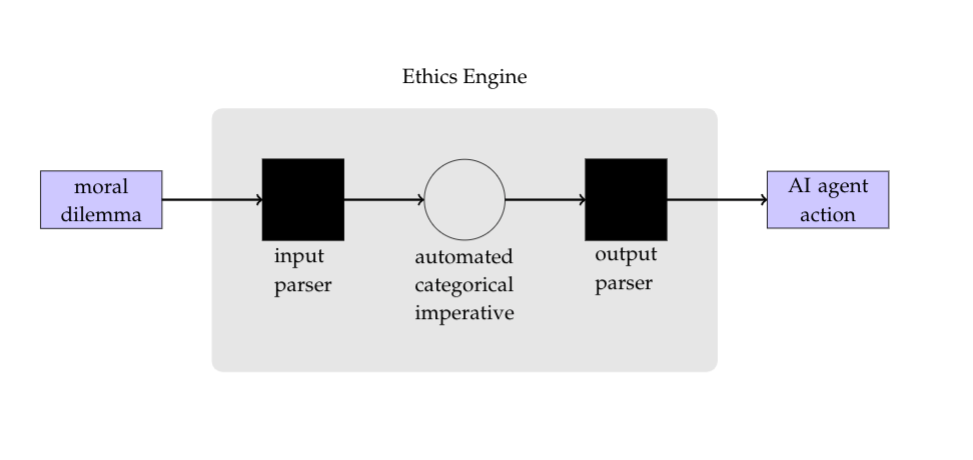
\includegraphics[scale=0.4]{AI_engine.png}
\caption{An example of an ethics engine for an artificial agent} \label{fig:AIengine}
\end{figure}
%
\begin{isamarkuptext}%
In this workflow, an AI agent is faced with a moral dilemma in some internal representation. This 
internal representation would need to be translated by an input parser into an appropriate logical representation, i.e. 
a circumstance, act, goal tuple. This input parser is the most technically and ethically challenging 
component of the system. It is this input parser that determines which circumstances are ``morally relevant"
for a maxim, a judgement that requires commonsense reasoning and knowledge about moral relevance. Much 
of the work that a Kantian human being does when making decisions is to translate everyday situations 
into appropriate maxims. Huge misunderstandings about Kantian ethics (maybe cite homophobia or right 
to lie) in the literature often result from incorrectly formulated maxims, and the entire field of 
applied Kantian ethics is devoted to generating the right kinds of maxims to test. 

This representational
question will be one of the biggest hurdles to actually using my categorical imperative library 
in an AI ethics engine. Currently, it may be reasonable for a human being to perform the role of the input
parser. Once an AI agent stumbles onto an ethical dilemma, a human being could take over, formulate 
the right question, and feed it into the categorical imperative library to see what action the categorical 
imperative would prescribe. This may actually be a feature, not a bug, of an ethics engine for AI. 
Proponents of the ``human-in-the-loop" model argue that fully automated decision-making is doomed 
to ethical failure, and that the inclusion of a human being injects common-sense sanity into otherwise 
dangerous decisions\footnote{maybe i should like...read a book}. 

It is likely that, regardless of the strengths of the human-in-the-loop model, fully automated AI 
agents will exist. Setting aside the question of whether or not developing this kind of AI is responsible,
such developments will require ethics engines, or risk no consideration of ethics at all. Even if a 
world of fully automated AI is scary, such a world with automated ethics is better than a world without. 
In such a world, the input parser in my ethics engine would have to be automated. This would require 
that the parser translate the AI agent's internal representation to the appropriate logical representation.
The input parser would need enough common sense reasoning to determine what circumstances are morally 
relevant to a maxim. This is a question that, like all of ethics, philosophers debate robustly (cite the lit,
there's tons of it). It is likely that, just as different implementations of automated ethics choose 
a particular ethical theory and implement it, different implementations of such an input parser would 
need to adopt different interpretations of commonsense reasoning and morally relevant circumstances.

Once the input has been parsed, either by a human or a machine, into  a sentence in my logic, my 
project can evaluate its moral status using my implementation of 
the FUL. Concretely, my project would return a value indicating if the maxim is obligatory, permissible, 
or prohibited. The maxim would be prohibited if it fails the universalizability test, permissible if it passes, and obligatory 
if its negation fails the universalizability test. All three of these properties amount to testing if a 
certain theorem holds or not in my logic, a calculation that I demonstrate in my tests. 

This output could then be converted into some actionable, useful response with another output parser, 
and then passed back to the AI agent. For example, if the AI agent is equipped to evaluate natural language prescriptions, the 
status of the maxim could be parsed into a natural language sentence. This output will be passed back 
to the AI agent, which will use it to make a decision. The input parser, categorical imperative library, 
and output parser together constitute an ``ethics engine" that AI agents could use as a black box 
implementation of an ethical theory. 

The ethics engine depicted above is a high-level example of one way to use my project to guide an artifical agent. The 
upshot is that an automated version of the categorical imperative could function as the ethical engine 
for an AI agent, with much work to parse the input and the output. Effectively, the kind 
of automated ethics I implement could be 
an ``ethics library" that AI developers could use to give AI agents the capacity for 
sophisticated ethical reasoning faithful to philosophical literature. This represents an improvement 
over existing ethics engines, which rarely attempt to capture the complexity 
of any ethical theory that philosophers plausibly defend. For more on how my project is situated 
among other work in automated ethics, see Section ??%
\end{isamarkuptext}\isamarkuptrue%
%
\isadelimdocument
%
\endisadelimdocument
%
\isatagdocument
%
\isamarkupsubsection{Computational Philosophy%
}
\isamarkuptrue%
%
\endisatagdocument
{\isafolddocument}%
%
\isadelimdocument
%
\endisadelimdocument
%
\begin{isamarkuptext}%
Above I explained how my system offers a mechanism for humans to build ethical AI agents. I also 
argue that computational ethics is a mechanism for computers to help humans think differently about 
philosophy. Just as theorem provers make mathematics more efficient and push mathematicians to think 
precisely about the phenomena they are modelling, computational ethics can help philosophers think about 
philosophy. Below I share an example of the kind of philosophical insight that computational ethics 
can prompt and analyze the value that this tool offers to philosophers.%
\end{isamarkuptext}\isamarkuptrue%
%
\isadelimdocument
%
\endisadelimdocument
%
\isatagdocument
%
\isamarkupsubsubsection{Example of a  Philosophical Insight%
}
\isamarkuptrue%
%
\endisatagdocument
{\isafolddocument}%
%
\isadelimdocument
%
\endisadelimdocument
%
\begin{isamarkuptext}%
The process of implementing and testing a formalization using an interactive theorem prover 
resulted in logical insights that led to a philosophical 
insight that was novel to me and is potentially novel to the field. This philosophical insight has
implications for what kinds of principles a practical reasoner should be concerned with. While this 
insight could have been reached without the help of the computer, my system's logical results provoked
an interesting philosophical conversation as I tried to understand their implications for the ethical 
theory I am formalizing. This serves as an example for how computational ethics can prompt philosophical 
insights. 

As I was implementing my formalization of the FUL, I realized
that my formalization was inconsistent unless I specified that the FUL only held for ``well-formed maxims,"
such that neither the act nor goal were already achieved in the given circumstances. Precisely, 
a circumstance, act, goal tuple (c, a, g) is well-formed if $(\neg (c \longrightarrow a) ) \wedge 
(\neg(c \longrightarrow g))$. This provoked the philosophical insight that maxims of this form, in which 
the act or the goal has already been accomplished in the given circumstances are ``vacuous" because 
any prescriptions they generate have already been acted on or violated. Below I document how I came 
to this conclusion and explain the notion of a vacuous maxim in greater detail.

\emph{Logical Insight}

First, I used Sledgehammer to show that my formalization of the FUL\footnote{The full logical representation is \isa{FUL{\isadigit{0}}\ {\isasymequiv}\ {\isasymforall}c\ a\ g\ s{\isachardot}\ not{\isacharunderscore}universalizable\ {\isacharparenleft}c{\isacharcomma}\ a{\isacharcomma}\ g{\isacharparenright}\ s\ {\isasymlongrightarrow}\ {\isasymTurnstile}prohibited\ {\isacharparenleft}c{\isacharcomma}\ a{\isacharcomma}\ g{\isacharparenright}\ s}.}
resulted in a contradiction. Sledgehammer was able to tell me which axioms it used to complete 
this proof, showing me that my formalization contradicted the axiom O\_diamond, which states that an 
obligated term cannot contradict its context\footnote{The full form of the axiom is 
$ O { A \vert B } \longrightarrow \diamond (B \wedge A)$}. 
O\_diamond formalizes the principle ``ought implies can" and requires that if A is obligated in context 
C, that A is possible in context C. I hypothesized that there was some tension between 
the antecedent of the FUL, which states that all agents act on the maxim, and the consequent, 
which states that the maxim is prohibited. If the maxim has already been acted on, then not acting on it
is impossible so the prohibition is impossible to obey so the ought implies can principle is violated, 
thus contradicting the axiom O\_diamond.

To solve this problem, I returned to Korsgaard's practical contradiction interpretation and focused 
on the imaginatory component of the FUL. Specifically, the universalizability test requires that we imagine 
a world where the maxim is universalized and study that world to determine whether or not the maxim 
is obligatory in the actual world. For example, lying is not universalized in our current world, but to 
determine if lying is prohibited, we imagine a different world in which everyone lied. To capture this difference,
I implemented another version of the FUL under which  a maxim is prohibited at the current world $cw$ if, 
when universalized at any world $w$ it is rendered ineffective at $w$. I hypothesized that this would remove 
the contradiction found above. To test this new formalization, I used Nitpick, a model checker that 
quickly generates models that satisfy the given axioms and theorems. Usually, Nitpick can find a satisfying 
model to show that a logic is consistent in a matter of seconds, but Nitpick consistently timed out 
when looking for a model of my modified FUL. 

Nitpick performs an optimized version of a brute force model search, in which it generates many models 
and checks if they satisfy the given maxims. I suspected that Nitpick 
was  timing out due to checking large models that exhausted its 
time limit, especially due to the logical complexity of my theory\footnote{Benzmueller warned me that as 
I added quantifiers to the theory, Isabelle's automated proof tools may start to time out.}. 
To reduce the logical complexity, I decided to specify the exact number of maxims 
in the system by passing as an argument to Nitpick the cardinality of my desired model. This did not 
fix the problem. 

I next defined a particular (circumstance, act, goal) tuple as a constant and, instead of
stating that the FUL held for all maxims, I stated that the FUL held for the specific maxim formed by this tuple.
While before I added the axiom $\forall (c, a, g). FUL holds for maxim = (c, a, g)$, I now added constants $(c, a, g)$ 
and added the axiom $FUL holds for maxim = (c, a, g)$. By specifying the circumstance, act, and goal 
as constants, I removed the external universal quantifier, thus removing a layer of logical complexity.

To my surprise, Nitpick was now able to show that the FUL was consistent!

This result was counterintuitive—after all, what is the difference between a model of cardinality 
1 and a model with one constant object? Why is quantifying over a tiny number of maxims so much 
more time-cosuming than analyzing a single maxim? Professor Amin pointed out that when I defined the 
circumstances, act, and goal as constants, then they were all distinct. When they were quantified over, 
they could be identical. To formalize this idea, I defined a maxim as ``well-formed" if \isa{well{\isacharunderscore}formed\ {\isasymequiv}\ {\isasymlambda}{\isacharparenleft}c{\isacharcomma}\ a{\isacharcomma}\ g{\isacharparenright}\ s\ w{\isachardot}\ {\isasymnot}\ c\isactrlbold {\isasymrightarrow}g\ w\ {\isasymand}\ {\isasymnot}\ c\isactrlbold {\isasymrightarrow}a\ s\ w}. In propositional 
logic, a circumstance, act, goal tuple (c, a, g) is well-formed if $(\neg (c \longrightarrow a) ) \wedge 
(\neg(c \longrightarrow g))$. I tested my hypothesis by modifying my axiom to instead read $\forall maxim
(maxim is well-formed \longrightarrow FUL holds for maxim)$. This version of the FUL was indeed inconsistent!

To summarize, I realized that my initial attempt at formalizing the FUL was inconsistent because 
it required that the FUL hold for badly formed maxims, in which the circumstances entail the act or 
goal. The logical insight was that if FUL holds for maxims in which $(c \longrightarrow a) \vee 
(c \longrightarrow g)$, then the logic will be inconsistent.

\emph{Philosophical Insight}

Once I realized this logical property, I tried to understand its philosophical plausibility. I define
a vacuous maxim as one in which the circumstances entail either the act or the goal. An example
of a vacuous maxim is: ``When eating breakfast, eat breakfast in order to eat breakfast." This 
maxim isn't clearly obligatory or prohibited, but there is something empty about it. For one 
thing, acting on this maxim would never result in any actual action. If an agent adopts this maxim, 
they decide that, in the circumstances ``eating breakfast" they will perform the act ``eating breakfast"
for the purpose ``eating breakfast." In these circumstances, the act has 
already been performed! Making this maxim a rule to live by doesn't change how you live your life. 
When you are eating breakfast, you eat breakfast, but this statement is already 
tautologically true regardless of whether you adopt the maxim or not. 

Not only does a badly formed maxim fail to prescribe action, any obligations or prohibitions it 
generates have already been fulfilled or violated and are thus foregone conclusions. If a badly formed 
maxim generates a prohibition, then this prohibition would be impossible to obey. 
It is impossible to not eat breakfast while eating breakfast, because the circumstances assume that the 
act has happened. On the other hand, if a badly formed maxim generates an obligation, then the obligation 
will have already been fulfilled. If you are required to eat breakfast while eating breakfast, then you've 
already fulfilled your obligation because the circumstances assume that the act has happened. Thus, 
a badly formed maxim does not actually guide action because it doesn't generate new obligations or 
prohibitions that could ever be acted on. 

The implication is that any obligations or prohibitions generated by a badly formed maxim are foregone 
conclusions and thus do not tell us how to live, and thus must not be the domain of ethics, because 
ethics is supposed to tell us how to live. Kant's categorical imperative
 guides our use of practical reason, which is the kind of reason that tells us what we should do. 
A practical reasoner asks moral questions not because they're mental puzzles or out of curiosity, but 
because the reasoner wants to know how to act. Practical reason is action-guiding, but a badly formed
 maxim can never be action-guiding because it prescribes no new
actions or obligations. It is not the kind of maxim that a practical reasoner would consider. 
There is no explicit prohibition against a badly formed maxim like the breakfast example above, but it 
is the wrong kind of question for a practical reasoner to ask. Moreover, an ordinary person trying 
to navigate the world would never ask that kind of question. If ethics and practical reason are meant 
to guide action, then badly formed maxims are not questions for ethics, because they could never guide 
action.

Above I show that badly formed maxims are not questions for the ethics, but they also represent a 
stronger problem. Asking if you should be acting while you act is undermining your will. 
Under the Kantian acount of willing, when you will a maxim, you make it your end and commit yourself 
to be its cause. You cannot simultaneously will a maxim and ask if you should be willing it. To say that 
you are willing the maxim is to say that you have decided to will it—so the question, ``should I be 
willing this?" is nonsensical. Either you haven't actually adopted the maxim, or you aren't
actually asking the question. In a badly formed maxim, the circumstances already assume that the agent 
has willed the maxim. If someone asks me``should I eat breakfast while eating breakfast?" I not only 
wouldn't be able to answer the question, I wouldn't understand what they're asking. I would say, ``what 
do you mean? You ARE eating breakfast." The agent must either not actually be eating breakfast or 
they must not be asking a real question. 

That being said, we do often ask ``should I be doing this?" as we do something. What do we mean when 
we ask this question? In what sense are we trying to evalute the moral status of a badly formed maxim?
Can this kind of question ever be valid? To understand this worry, I consider the maxim, 
``When dancing, I should just dance for the sake of dancing."\footnote{Maybe cite Korgsaard since the
dancing thing is her example.} While this maxim appears to be badly formed (the 
circumstance `dancing' implies the act and goal), it's a question that practical reasoners 
do ask. I argue that there are multiple ways of understanding this maxim, and none are inconsistent with 
my complaints about badly formed maxims. 

First is what I call the ``different action" interpretation, under which "I should just dance" is 
actually referring to a different act than the circumstances. The circumstances ``When dancing" refer 
to rythmically moving your body to music, but ``I should just dance" refers to dancing without anxiety, 
completely focused on the joy of dancing itself. More precisely, this maxim should actually read ``When 
dancing, I should abandon my anxiety and focus on dancing for the sake of dancing." This maxim when so 
modified is not vacuous at all—abandoning anxiety and focusing on dancing is an entirely different act 
from moving your body rythmically to music. This maxim is thus actually well-formed, and thus doesn't
pose a problem for my argument. It is entirely plausible to tell yourself ``When I am dancing, I should focus 
on dancing for the sake of dancing itself." The circumstances do not entail the act or the goal because 
they refer to different meanings of the word dancing. 

Another version of the ``different action" interpretation is as follows. Consider the maxim modified to 
be ``When dancing and seeing a child drowning, I should dance for the sake of dancing." Clearly this 
maxim is fit for moral evaluation, and we expect a moral theory to prohibit this maxim. The circumstances 
``When dancing and seeing a child drowning" appear to entail the act of dancing. In this case, the question 
that the agent is actually asking themselves is ``should I continue dancing?" That is the actionable 
maxim that they will adopt or reject. They mean to ask if they should stop dancing and go help the child. 
Dancing at the current moment and dancing at the next moment are different acts, and the circumstances 
imply the former but not the latter. A badly formed maxim would have circumstances and act both 
``dancing at moment t," but this maxim has circumstances ``dancing at moment t" and act ``dancing 
at moment t+1."

Another interpretation of the dancing example is the ``self doubt" intepretation. The question ``When I am dancing, 
should I really be dancing for the sake of dancing?" is the agent asking, ``Am I doing the right thing 
right now?" The agent is not asking about the next moment, but is expressing doubt about the 
moral validity of their behavior at this current moment. Under this interpretation, the agent 
wants to know if they made the right decision. But what decision has the agent made? Did the agent
adopt the maxim ``When dancing, dance for the sake of dancing?" They could not have, because such a 
maxim could not have altered their behavior at all. This agent actually wants to know if the maxim that 
resulted in them dancing, the maxim that got them to the current moment on the dance floor, was actually 
the right thing to do. They are asking if, in the past, when they decided to dance, they made the 
right decision. But such a maxim is not vacuous, because it resulted in the act of dancing. 
The maxim that initiated the dancing would be something like ``When at a wedding, dance for the sake 
of dancing." This is the maxim that they are currently acting on, not the badly formed example maxim.
Evaluating the moral validity of this maxim is straightforward.

This analysis also demonstrates the correct way to think about moral regret and self-doubt. When we 
ask ``should I really be doing this?" we are asking if, when we chose to adopt our current maxim, 
we made the right decision. The question is not, ``When acting should I act?" The question is, ``When 
I was in the past, should I have chosen to act?" Regret is a counterfactual question about a valid, 
well-formed maxim that was adopted in the past and led to the present moment. Unlike a badly formed 
maxim, it doesn't undermine the will because it acknowledges the will's authority and the fact that the 
will made a decision, but it asks if the will was mistaken.%
\end{isamarkuptext}\isamarkuptrue%
%
\isadelimdocument
%
\endisadelimdocument
%
\isatagdocument
%
\isamarkupsubsubsection{The Value of Computational Ethics%
}
\isamarkuptrue%
%
\endisatagdocument
{\isafolddocument}%
%
\isadelimdocument
%
\endisadelimdocument
%
\begin{isamarkuptext}%
I do not argue that computational ethics, as it stands today, uncovers philosophical insights that humans have not reached 
or are incapable of reaching. After all, my understanding of a well-formed maxim could 
very well exist in the literature and certainly could be reached by a philosopher working without any 
computational tools. Instead, I argue that computational tools prompt philosophers to ask questions that 
lead to insights. Philosophers already value precision, and the computer forces precision and makes formal
reasoning easier. Computational 
ethics can serve as another tool in a philosopher's arsenal, like a thought experiment or counterexample.
While the technology is not yet mature enough and easy enough to use to become widespread in philosophy
departments, technical progress could turn computational ethics into an easy-to-use tool for philosophers
that doesn't require any specialized knowledge.

The first contribution of computational ethics is precision. Much of analytic philosophy involves 
making a particular concept precise. Thought experiments, arguments, counterexamples, and examples 
illustrate features of a concept in the hope of making the concept itself more precise. Computational 
ethics can help philosophers reach this goal of precision in another, potentially easier, way. 
Representing a philosophical idea in logic and implementing it in an interactive theorem prover requires 
making the idea precise to a degree that ordinary discussion can result in, but does not necessarily require. The initial representation 
of an idea in a logic requires making its form precise. For example, 
as I formalized the notion of a maxim, I had to understand its components and define it as a 
circumstance, act, goal tuple. Moreover, Isabelle's strict typing system required that I define 
coherent, consistent types for each of these entities and for a maxim as a whole. This requires understanding 
what role each of these components play in the FUL and assigning them each a type. In my example, I 
concluded that circumstances and goals are terms, which can be true or false at a world, and acts are 
open sentences, which are true for a particular subject at a particular world. This precision is possible 
without computational tools, but computational ethics forces a level of precision that ordinary discussion 
does not demand. Type fuzziness and overloaded definitions are all too common in philosophical writing and 
discussion (would be cool to cite some famous debate revolving around this idea), but computers don't 
allow this kind of imprecision.

Another, related benefit of computational ethics is that it makes formal ethics far less tedious. 
Certain subfields, such as philosophy of language, see such benefit in precision that they already heavily 
use symbolic logic to represent philosophical concepts, just as mathematicians use symbolic logic to 
represent mathematical concepts. Some of this work requres tedious pencil and paper proofs to prove 
theorems, even when many of these theorems may not generate relevant philosophical insights. Ineractive 
theorem provers make proofs more accessible. Isabelle can complete a proof, starting from first principles, 
in a matter of seconds that would take a logician pages to complete. Just as calculators make arithmetic 
more accessible, computational ethics does the same for formal philosophy. Not all philosophy can or will 
be automated—after all, calculators didn't make accountants or mathematicians obsolete. Just as computers 
reduce the tedium in other aspects of our life, they can reduce the tedium involved in formal logic for 
both mathematicians and philosophers.%
\end{isamarkuptext}\isamarkuptrue%
%
\isadelimdocument
%
\endisadelimdocument
%
\isatagdocument
%
\isamarkupsubsubsection{Looking Forward%
}
\isamarkuptrue%
%
\endisatagdocument
{\isafolddocument}%
%
\isadelimdocument
%
\endisadelimdocument
%
\begin{isamarkuptext}%
Computational ethics is at its infancy. The use of theorem provers in mathematics is just now beginning 
to make headway \cite{buzzardvideo}, even though theorem provers were first invented in the 1960's \cite{historyofITP}. In contrast, the first attempts to use theorem 
provers for ethics occurred in the last decade. The fact that this nascent technology is already 
helping humans reach non-trivial philosophical conclusions is reason to, at the very least, entertain 
the possibility of a future where computational ethics becomes as normal for philosophers.

To the skeptic, the ethical insights uncovered by the computer are not necessarily impressive 
philosophy. Indeed, the fact that a theorem prover requires specialized knowledge outside of the field 
of philosophy indicates that the technology is nowhere near ready for universal use in philosophy 
departments. However, history indicates that as computing power increases and computer scientists make 
progress, computational ethics will become more usable. Theorem provers in mathematics began as toys 
incapable of proving that the real number 2 is not equal to the real number 1, but Buzzard showed that 
moving from such a primitive system to a tool for Fields medal winning mathematics is possible in a 
matter of years \cite{buzzardvideo}. Countless examples from the history of computer science, from the Turing 
Test to AI game playing to protein folding, demonstrate that progress in computer science can make seemingly 
obscure computer programs useful and usable in ways that exceed our wildest imaginations. Indeed, 
programmable computers themselves initially began as unwieldy punch card readers, but their current ubiquity 
need not be stated. If computer scientists and philosophers invest in computational ethics, it can 
become as much a tool for philosophy as a calculator is for for arithmetic.\footnote{Is this too like, 
lalalala fantasy of computational philosophy? Would it be less so if I did more work explaining 
the history of theorem proving for math? Is this even that important for my project?}%
\end{isamarkuptext}\isamarkuptrue%
%
\isadelimtheory
%
\endisadelimtheory
%
\isatagtheory
%
\endisatagtheory
{\isafoldtheory}%
%
\isadelimtheory
%
\endisadelimtheory
%
\end{isabellebody}%
\endinput
%:%file=~/Desktop/cs91r/paper/upshot.thy%:%
%:%24=6%:%
%:%36=8%:%
%:%37=9%:%
%:%38=10%:%
%:%39=11%:%
%:%40=12%:%
%:%41=13%:%
%:%42=14%:%
%:%43=15%:%
%:%44=16%:%
%:%53=18%:%
%:%65=20%:%
%:%66=21%:%
%:%67=22%:%
%:%68=23%:%
%:%69=24%:%
%:%70=25%:%
%:%71=26%:%
%:%72=27%:%
%:%73=28%:%
%:%74=29%:%
%:%75=30%:%
%:%76=31%:%
%:%77=32%:%
%:%78=33%:%
%:%81=37%:%
%:%82=38%:%
%:%83=39%:%
%:%84=40%:%
%:%85=41%:%
%:%88=43%:%
%:%89=44%:%
%:%90=45%:%
%:%91=46%:%
%:%92=47%:%
%:%93=48%:%
%:%94=49%:%
%:%95=50%:%
%:%96=51%:%
%:%97=52%:%
%:%98=53%:%
%:%99=54%:%
%:%100=55%:%
%:%101=56%:%
%:%102=57%:%
%:%103=58%:%
%:%104=59%:%
%:%105=60%:%
%:%106=61%:%
%:%107=62%:%
%:%108=63%:%
%:%109=64%:%
%:%110=65%:%
%:%111=66%:%
%:%112=67%:%
%:%113=68%:%
%:%114=69%:%
%:%115=70%:%
%:%116=71%:%
%:%117=72%:%
%:%118=73%:%
%:%119=74%:%
%:%120=75%:%
%:%121=76%:%
%:%122=77%:%
%:%123=78%:%
%:%124=79%:%
%:%125=80%:%
%:%126=81%:%
%:%127=82%:%
%:%128=83%:%
%:%129=84%:%
%:%130=85%:%
%:%131=86%:%
%:%132=87%:%
%:%133=88%:%
%:%134=89%:%
%:%135=90%:%
%:%136=91%:%
%:%137=92%:%
%:%138=93%:%
%:%139=94%:%
%:%140=95%:%
%:%141=96%:%
%:%142=97%:%
%:%151=99%:%
%:%163=101%:%
%:%164=102%:%
%:%165=103%:%
%:%166=104%:%
%:%167=105%:%
%:%168=106%:%
%:%177=108%:%
%:%189=110%:%
%:%190=111%:%
%:%191=112%:%
%:%192=113%:%
%:%193=114%:%
%:%194=115%:%
%:%195=116%:%
%:%196=117%:%
%:%197=118%:%
%:%198=119%:%
%:%199=120%:%
%:%200=121%:%
%:%201=122%:%
%:%202=123%:%
%:%203=124%:%
%:%204=125%:%
%:%205=126%:%
%:%206=127%:%
%:%207=128%:%
%:%208=129%:%
%:%209=130%:%
%:%210=131%:%
%:%211=132%:%
%:%212=133%:%
%:%213=134%:%
%:%214=135%:%
%:%215=136%:%
%:%216=137%:%
%:%217=138%:%
%:%218=139%:%
%:%219=140%:%
%:%220=141%:%
%:%221=142%:%
%:%222=143%:%
%:%223=144%:%
%:%224=145%:%
%:%225=146%:%
%:%226=147%:%
%:%227=148%:%
%:%228=149%:%
%:%229=150%:%
%:%230=151%:%
%:%231=152%:%
%:%232=153%:%
%:%233=154%:%
%:%234=155%:%
%:%235=156%:%
%:%236=157%:%
%:%237=158%:%
%:%238=159%:%
%:%239=160%:%
%:%240=161%:%
%:%241=162%:%
%:%242=163%:%
%:%243=164%:%
%:%244=165%:%
%:%245=166%:%
%:%246=167%:%
%:%247=168%:%
%:%248=169%:%
%:%249=170%:%
%:%250=171%:%
%:%251=172%:%
%:%252=173%:%
%:%253=174%:%
%:%254=175%:%
%:%255=176%:%
%:%256=177%:%
%:%257=178%:%
%:%258=179%:%
%:%259=180%:%
%:%260=181%:%
%:%261=182%:%
%:%262=183%:%
%:%263=184%:%
%:%264=185%:%
%:%265=186%:%
%:%266=187%:%
%:%267=188%:%
%:%268=189%:%
%:%269=190%:%
%:%270=191%:%
%:%271=192%:%
%:%272=193%:%
%:%273=194%:%
%:%274=195%:%
%:%275=196%:%
%:%276=197%:%
%:%277=198%:%
%:%278=199%:%
%:%279=200%:%
%:%280=201%:%
%:%281=202%:%
%:%282=203%:%
%:%283=204%:%
%:%284=205%:%
%:%285=206%:%
%:%286=207%:%
%:%287=208%:%
%:%288=209%:%
%:%289=210%:%
%:%290=211%:%
%:%291=212%:%
%:%292=213%:%
%:%293=214%:%
%:%294=215%:%
%:%295=216%:%
%:%296=217%:%
%:%297=218%:%
%:%298=219%:%
%:%299=220%:%
%:%300=221%:%
%:%301=222%:%
%:%302=223%:%
%:%303=224%:%
%:%304=225%:%
%:%305=226%:%
%:%306=227%:%
%:%307=228%:%
%:%308=229%:%
%:%309=230%:%
%:%310=231%:%
%:%311=232%:%
%:%312=233%:%
%:%313=234%:%
%:%314=235%:%
%:%315=236%:%
%:%316=237%:%
%:%317=238%:%
%:%318=239%:%
%:%319=240%:%
%:%320=241%:%
%:%321=242%:%
%:%322=243%:%
%:%323=244%:%
%:%324=245%:%
%:%325=246%:%
%:%326=247%:%
%:%327=248%:%
%:%328=249%:%
%:%329=250%:%
%:%330=251%:%
%:%331=252%:%
%:%332=253%:%
%:%333=254%:%
%:%334=255%:%
%:%335=256%:%
%:%336=257%:%
%:%337=258%:%
%:%338=259%:%
%:%339=260%:%
%:%340=261%:%
%:%341=262%:%
%:%342=263%:%
%:%343=264%:%
%:%344=265%:%
%:%345=266%:%
%:%346=267%:%
%:%347=268%:%
%:%348=269%:%
%:%349=270%:%
%:%350=271%:%
%:%351=272%:%
%:%352=273%:%
%:%353=274%:%
%:%354=275%:%
%:%355=276%:%
%:%356=277%:%
%:%357=278%:%
%:%358=279%:%
%:%359=280%:%
%:%360=281%:%
%:%361=282%:%
%:%362=283%:%
%:%363=284%:%
%:%364=285%:%
%:%373=288%:%
%:%385=290%:%
%:%386=291%:%
%:%387=292%:%
%:%388=293%:%
%:%389=294%:%
%:%390=295%:%
%:%391=296%:%
%:%392=297%:%
%:%393=298%:%
%:%394=299%:%
%:%395=300%:%
%:%396=301%:%
%:%397=302%:%
%:%398=303%:%
%:%399=304%:%
%:%400=305%:%
%:%401=306%:%
%:%402=307%:%
%:%403=308%:%
%:%404=309%:%
%:%405=310%:%
%:%406=311%:%
%:%407=312%:%
%:%408=313%:%
%:%409=314%:%
%:%410=315%:%
%:%411=316%:%
%:%412=317%:%
%:%413=318%:%
%:%414=319%:%
%:%415=320%:%
%:%416=321%:%
%:%417=322%:%
%:%418=323%:%
%:%419=324%:%
%:%420=325%:%
%:%421=326%:%
%:%422=327%:%
%:%423=328%:%
%:%424=329%:%
%:%433=332%:%
%:%445=335%:%
%:%446=336%:%
%:%447=337%:%
%:%448=338%:%
%:%449=339%:%
%:%450=340%:%
%:%451=341%:%
%:%452=342%:%
%:%453=343%:%
%:%454=344%:%
%:%455=345%:%
%:%456=346%:%
%:%457=347%:%
%:%458=348%:%
%:%459=349%:%
%:%460=350%:%
%:%461=351%:%
%:%462=352%:%
%:%463=353%:%
%:%464=354%:%
%:%465=355%:%